%-------------------------------------------------------------------------------
% This file provides a skeleton ATLAS document
%-------------------------------------------------------------------------------
\documentclass[UKenglish,texlive=2011]{latex/atlasdoc}
% The language of the document must be set: usually UKenglish or USenglish
% british and american also work!
% Selected options:
%  texlive=YYYY          Specify TeX Live version (2013 is default)
%  atlasstyle=true|false Use ATLAS style for document (default)
%  coverpage             Create ATLAS draft cover page for collaboration circulation
%                        See atlas-draft-cover.tex for a list of variables that should be defined.
%  cernpreprint          Create front page for a CERN preprint
%                        See atlas-preprint-cover.tex for a list of variables that should be defined.
%  PAPER                 The document is an ATLAS paper (draft)
%  CONF                  The document is a CONF note (only useful together with coverpage)
%  PUB                   The document is a PUB note (only useful together with coverpage)
%  txfonts=true|false    Use txfonts rather than the default newtx - needed for arXiv submission
%  paper=a4|letter       Set paper size to A4 (default) or letter
%  maketitle=true|false  Run or do not run \maketitle from the class

%-------------------------------------------------------------------------------
% Extra packages:
\usepackage{latex/atlaspackage}
\usepackage{listings}
\definecolor{listinggray}{gray}{0.9}
\definecolor{lbcolor}{rgb}{0.9,0.9,0.9}
\definecolor{Green}{rgb}{0, 0.5, 0}
\lstset{
	backgroundcolor=\color{lbcolor},
    tabsize=4,    
%   rulecolor=,
    language=[GNU]C++,
    captionpos=b,
    basicstyle=\scriptsize,
    upquote=true,
    aboveskip={0.25\baselineskip},%{1.5\baselineskip},
    columns=fixed,
    showstringspaces=false,
    extendedchars=false,
    breaklines=true,
	prebreak = \,\,\,\,,%\raisebox{0ex}[0ex][0ex]{\ensuremath{\hookleftarrow}},
    frame=lines,%single,
    numbers=left,
    numberstyle=\tiny,
    numbersep=1.5pt,
    showtabs=false,
    showspaces=false,
    showstringspaces=false,
    identifierstyle=\ttfamily,%\color{magenta},
    keywordstyle=\color[rgb]{0,0,1},
    commentstyle=\color{Green},
    stringstyle=\color{red},
%    numberstyle=\color[rgb]{0.205, 0.142, 0.73},
    numberstyle=\color[RGB]{139, 69, 19},
%   \lstdefinestyle{C++}{language=C++,style=numbers}’.
}

% Selected options:
%  biblatex=true|false   Use biblatex (default) or bibtex for the bibliography
%  backend=biber         Use the biber backend rather than bibtex
%  minimal               Minimal set of packages
%  default               Standard set of packages
%  full                  Full set of packages
% Style file with biblatex options for ATLAS documents
\usepackage{latex/atlasbiblatex}

% Package for creating list of authors and contributors to the analysis
\usepackage{latex/atlascontribute}

% Useful macros
\usepackage{latex/atlasphysics}
% See doc/atlas-physics.pdf for a list of the defined symbols
% Default options are 
%   true:  journal, misc, particle, unit, xref
%   false: bsm, hion, math, process, other, texmf
% See the package for details on the options

% Files with references for use with biblatex
% Note that biber gives an error if it finds empty bib files
\addbibresource{universality2019.bib}
% \addbibresource{bibtex/bib/ATLAS.bib}
% \addbibresource{bibtex/bib/PubNotes.bib}
% \addbibresource{bibtex/bib/ConfNotes.bib}

% Paths for figures - do not forget the / at the end of the directory name
\graphicspath{{logos/}{figures/}}

% Add you own definitions here (file Isolation2017-defs.sty)
\usepackage{universality2019-defs}
\usepackage{rotating}

%-------------------------------------------------------------------------------
% Generic document information
%-------------------------------------------------------------------------------

% Author and title for the PDF file
\hypersetup{pdftitle={ATLAS draft},pdfauthor={The ATLAS Collaboration}}
% Title, abstract and document 
%-------------------------------------------------------------------------------
% This file contains the title, author and abstract.
% It also contains all relevant document numbers used by the different cover pages.
%-------------------------------------------------------------------------------

% Title
\AtlasTitle{Lepton (non)-universality in W decays in Run 2}

% Author - this does not work with revtex (add it after \begin{document})
% \author{The ATLAS Collaboration}

% Authors and list of contributors to the analysis
% \AtlasAuthorContribute also adds the name to the author list
% Include package latex/atlascontribute to use this
% Use authblk package if there are multiple authors, which is included by latex/atlascontribute
% \usepackage{authblk}
% \renewcommand\Authands{, } % avoid ``. and'' for last author
% \renewcommand\Affilfont{\itshape\small} % affiliation formatting
% \AtlasAuthorContributor{A Test}{b}{Author's contribution.}
\AtlasAuthorContributor{Nicolo de Groot}{a}{Some description what have been done.}
\AtlasAuthorContributor{Daniil Ponomarenko}{a,b}{Some description what have been done.}

\affil[a]{Radboud University}
\affil[b]{Moscow MEPhI}


% If a special author list should be indicated via a link use the following code:
% Include the two lines below if you do not use atlasstyle:
% \usepackage[marginal,hang]{footmisc}
% \setlength{\footnotemargin}{0.5em}
% Use the following lines in all cases:
% \usepackage{authblk}
% \author{The ATLAS Collaboration%
% \thanks{The full author list can be found at:\newline
%   \url{https://atlas.web.cern.ch/Atlas/PUBNOTES/ATL-PHYS-PUB-2014-007/authorlist.pdf}}
% }

% Date: if not given, uses current date
%\date{\today}

% Draft version:
% Should be 1.0 for the first circulation, and 2.0 for the second circulation.
% If given, adds draft version on front page, a 'DRAFT' box on top of each other page, 
% and line numbers.
% Comment or remove in final version.
\AtlasVersion{0.0}

% ATLAS reference code, to help ATLAS members to locate the paper
\AtlasRefCode{ATL-COM-PHYS-2019-XXX}

% ATLAS note number. Can be an COM, INT, PUB or CONF note
% \AtlasNote{ATLAS-CONF-2014-XXX}
% \AtlasNote{ATL-PHYS-PUB-2014-XXX}
% \AtlasNote{ATL-COM-PHYS-2014-XXX}

% CERN preprint number
% \PreprintIdNumber{CERN-PH-2014-XX}

% ATLAS date - arXiv submission; to be filled in by the Physics Office
% \AtlasDate{\today}

% arXiv identifier
% \arXivId{14XX.YYYY}

% HepData record
% \HepDataRecord{ZZZZZZZZ}

% Submission journal and final reference
% \AtlasJournal{Phys.\ Lett.\ B.}
% \AtlasJournalRef{\PLB 789 (2014) 123}
% \AtlasDOI{}

% Abstract - % directly after { is important for correct indentation
\AtlasAbstract{%
  Interesting hints of lepton non-universality have been seen in decays of B hadrons.  Measurements from LEP on W decays also show a hint of non universality at the level of a few percent. ATLAS has produced over $10^9$ W decays to leptons, which allows us to make a high-precision measurement of lepton (non)-universality in W decay by measuring the ratio $W\rightarrow \tau\nu \rightarrow \ell\nu\bar{\nu}$ / $W \rightarrow \ell\nu$ where $\ell = e,\mu$, in which many systematic effects cancel. Main challenges are control of the non-W background and trigger related systematics.
}


%-------------------------------------------------------------------------------
% The following information is needed for the cover page. The commands are only defined
% if you use the coverpage option in atlasdoc or use the atlascover package
%-------------------------------------------------------------------------------

% List of supporting notes  (leave as null \AtlasCoverSupportingNote{} if you want to skip this option)
% \AtlasCoverSupportingNote{Short title note 1}{https://cds.cern.ch/record/XXXXXXX}
% \AtlasCoverSupportingNote{Short title note 2}{https://cds.cern.ch/record/YYYYYYY}
%
% OR (the 2nd option is deprecated, especially for CONF and PUB notes)
%
% Supporting material TWiki page  (leave as null \AtlasCoverTwikiURL{} if you want to skip this option)
% \AtlasCoverTwikiURL{https://twiki.cern.ch/twiki/bin/view/Atlas/WebHome}

% Comment deadline
% \AtlasCoverCommentsDeadline{DD Month 2014}

% Analysis team members - contact editors should no longer be specified
% as there is a generic email list name for the editors
% \AtlasCoverAnalysisTeam{Peter Analyser, Susan Editor1, Jenny Editor2, Alphonse Physicien}

% Editorial Board Members - indicate the Chair by a (chair) after his/her name
% Give either all members at once (then they appear on one line), or separately
% \AtlasCoverEdBoardMember{EdBoard~Chair~(chair), EB~Member~1, EB~Member~2, EB~Member~3}
% \AtlasCoverEdBoardMember{EdBoard~Chair~(chair)}
% \AtlasCoverEdBoardMember{EB~Member~1}
% \AtlasCoverEdBoardMember{EB~Member~2}
% \AtlasCoverEdBoardMember{EB~Member~3}

% A PUB note has readers and not an EdBoard -- give their names here (one line or several entries)
% \AtlasCoverReaderMember{Reader~1, Reader~2}
% \AtlasCoverReaderMember{Reader~1}
% \AtlasCoverEdBoardMember{Reader~2}

% Editors egroup
% \AtlasCoverEgroupEditors{atlas-GROUP-2014-XX-editors@cern.ch}

% EdBoard egroup
% \AtlasCoverEgroupEdBoard{atlas-GROUP-2014-XX-editorial-board@cern.ch}


% langage stuff
\newcommand{\ie}{{\it i.e.}}

%style stuff
\def\rs{\raisebox{1.3ex}[-1.5ex]}

% isolation stuff
\newcommand*{\rhomedian}{\ensuremath{\rho_{median}}\xspace}


%-------------------------------------------------------------------------------
% Content
%-------------------------------------------------------------------------------
\begin{document}

% \maketitle
\tableofcontents
\FloatBarrier

% List of contributors - print here or after the Bibliography
%\AtlasPrintContribute{0.3}

%-------------------------------------------------------------------------------
\section{Introduction}
\label{sec:intro}

Lepton universality is one of the cornerstones of the Standard Model of particle physics. 
In the past years interesting hints of lepton non-universality have been seen in semi-leptonic decays of B hadrons~\cite{HFLAV16} where an excess of $\tau$ final states over $e,\mu$ final states is seen at the level of 4 standard deviations .
Measurements from LEP on W decays also show a hint of non universality at the level of a few percent~\cite{LEP-2}, again with a surplus of $\tau$ final states: 
\begin{equation}
  \label{eq:LEP_BRoverBRAll}
  \frac{2Br(W\to\tau\nu)}{Br(W\to\mu\nu)+Br(W\to e\nu)} = 1.077 \pm 0.026
\end{equation}
resulting in a poor agreement at the level of 2.8 standard deviations, with all correlations included.

Both results are shown in Figure~\ref{fig:lnuhints}.

\begin{figure}[htbp]
\centering
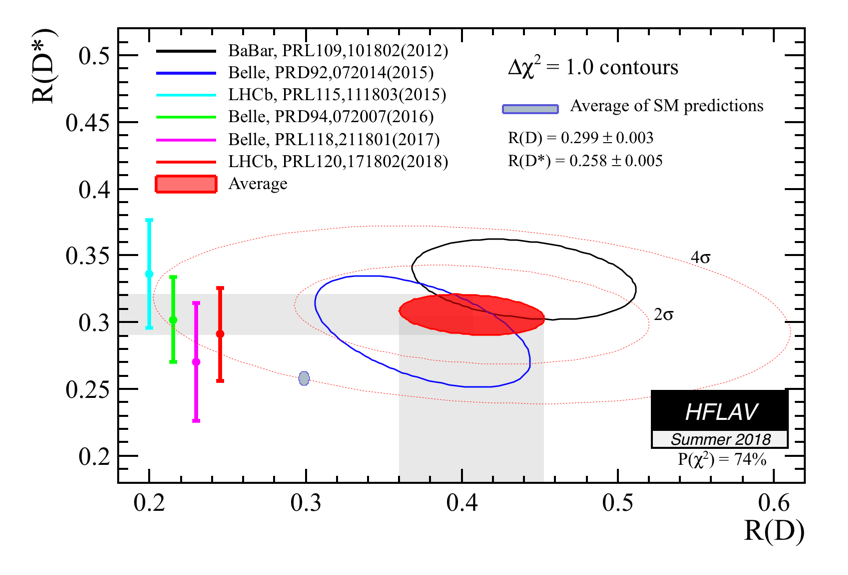
\includegraphics[width=10cm]{figures/rdrds_summer18.png}
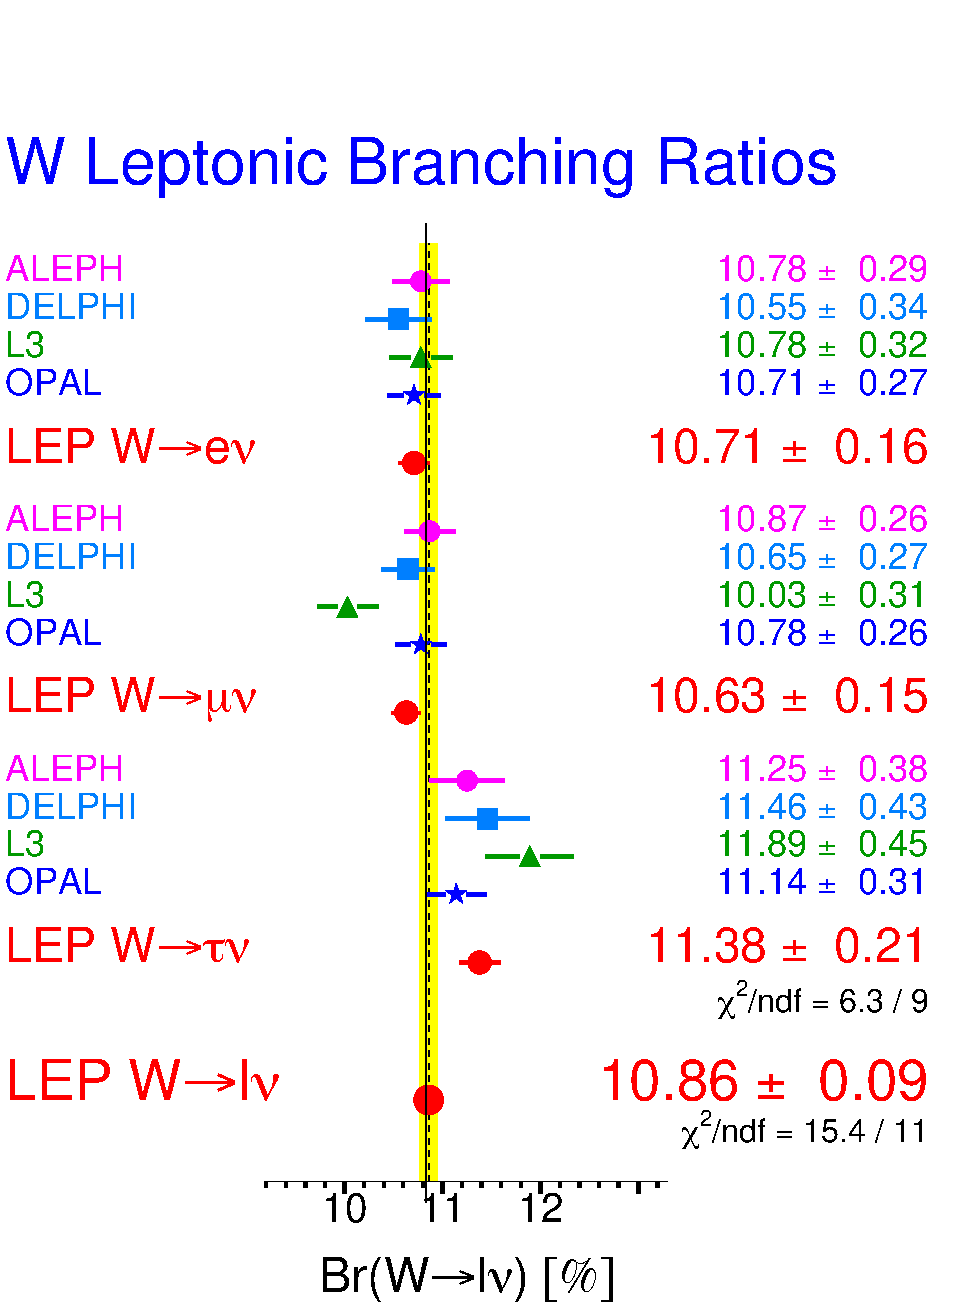
\includegraphics[width=6cm]{figures/4f_brlv_lep_2008.pdf}
\caption{\colorbox{yellow}{Left: Lepton universality in $B\to D^{(*)}$ decay from \cite{HFLAV16}. 
Right:  W leptonic branching ratios from \cite{LEP-2}}}
\label{fig:lnuhints}
\end{figure}

\subsection{Summary of the Analysis Strategy}
The ATLAS experiment has produced over $10^9$ W decays to leptons, which allows us to make a high-precision measurement of lepton (non)-universality in W decay by measuring the ratio $W\rightarrow \tau \rightarrow e/\mu$ / $W \rightarrow e/\mu$ in which many of the systematic effects related to lepton identification cancel. 
Most leptons will come from prompt $W$ decay since the branching fraction of tau to leptons is 17\% and many leptons coming from $W\to\tau\to \ell$ decay do not make it through the L1 trigger because of their lower momentum. 
Our first step will be to identify parts of the phase space enriched in tau decays using a multivariate classifier based on kinematic information and on the impact parameter of the lepton.
Since these to variables are largely uncorrelated we can constrain the efficiency from data.

Control regions are defined to constrain the modelling of the major backgrounds: $Z$ boson production and QCD fake leptons.


\FloatBarrier
%-------------------------------------------------------------------------------

%-------------------------------------------------------------------------------
\section{The ATLAS detector}
\label{sec:ATLAS}

The ATLAS experiment~\cite{Collaboration_2008} is a multi-purpose particle detector with a forward-backward symmetric cylindrical geometry and nearly $4\pi$ coverage in sold angle.
The collision point is surrounded by inner tracking devices followed by a superconducting solenoid providing a 2T magnetic field, a calorimeter system, and a muon spectrometer.

The inner tracker provides precision tracking of charged particles for pseudorapidities $|\eta|<2.5$.
It consists os pixel and silicon-microstrip detectors inside of a transition radiation tracker.
One significant upgrade for the new 13~TeV running period is the presence of the Insertable B-Layer~\cite{Capeans:1291633}, an additional pixel layer that provides high-resolution hits at small radius to improve tracking performance.

In the pseudorapidity region $|\eta|<3.2$, high-granularity lead/liquid-argon (LAr) electromagnetic (EM) sampling calorimeters are used.
An iron/scintillator tile calorimeter measures hadron energies for $|\eta|<1.7$.
The endcap and forward regions, spanning $1.5 < |\eta| < 4.9$, are instrumented with LAr calorimeters for both EM and hadronic measurements.

The muon spectrometer consists of three large superconducting toroids with 8 coils each, a system of trigger chambers, and precision tracking chambers,  which provide triggering and tracking capabilities in the ranges $|\eta|<2.4$ and $|\eta|<2.7$, respectively.

The two level trigger system is used to select events.
The first-level trigger is implemented in hardware and uses a subset of the detector information.
This is followed by the software-based High-Level Trigger (HLT) system, which can run offline reconstruction and calibration software, reducing the event rate to less than 1 kHz.
\FloatBarrier
%-------------------------------------------------------------------------------

%-------------------------------------------------------------------------------
\section{Data and Monte Carlo samples}
\label{sec:samples}

%\colorbox{red}{The samples may need to be updated}

\subsection{Samples}
\label{subsec:samples}

The samples used in this note are \colorbox{yellow}{MC15} \SI{13}{\tera\electronvolt} reconstructed using release 21 that includes the most recent isolation computation and corrections. They are detailed in Table~\ref{tab:samples}.

\begin{table}[htbp]
\centering
\begin{tabular}{|c|c|l|c|}
\hline
Process & Dataset ID & Tags \\ %$N_{events}$ \\
\hline
$W \to \mu\nu$ & 364156 - 364169 & e5340\_s3126\_r9364\_r9315\_p3401 \\
$W \to e\nu$ & 364170 - 364183 & e5340\_s3126\_r9364\_r9315\_p3401 \\
$W \to \tau\nu$ & 364184 - 364197 & e5340\_s3126\_r9364\_r9315\_p3401 \\

$Z \to \ee$ & 361106 & e3601\_s3126\_r9364\_r9315\_p3401 \\
$Z \to \mumu$ & 361107 & e3601\_s3126\_r9364\_r9315\_p3401 \\
$Z \to \tautau$ & 361108 & e3601\_s3126\_r9364\_r9315\_p3401 \\
\ttbar & 410011 - 410015 & e3824\_s3126\_r9364\_r9315\_p3401 \\
 & 410025 - 410026 & e3824\_s3126\_r9364\_r9315\_p3401 \\
Diboson & 363355 - 363360 & e5525\_s3126\_r9364\_r9315\_p3401 \\
 & 363489 & e5525\_s3126\_r9364\_r9315\_p3401 \\
 
\hline
\end{tabular}
\caption{\colorbox{yellow}{TO BE UPDATED!}}
\label{tab:samples}
\end{table}


\subsection{Object selection and truth matching}
\label{subsec:objects}



\subsection{Pile-up in Monte Carlo samples}
\label{subsec:pusamples}


\FloatBarrier
%-------------------------------------------------------------------------------

%-------------------------------------------------------------------------------
\section{Object definition}
\label{sec:objectdef}

This section describes the definitions of the physics objects employed in the analysis (electron, muon, jets and missing transverse energy). For the kinematic variables used in the analysis, they are all calculated with respect to the primary vertex selected in the event.

\subsection{Leptons}

\subsubsection{Electron definition}

\subsubsection{Muon definition}

\subsection{Jets}
Jets are built from topological clusters, formed from calorimeter cell deposits, and calibrated to the electromagnetic (EM) scale. They are reconstructed using the anti-kt algorithm with a distance parameter of R = 0.4. The jet four-vector is then corrected for the beamspot and a jet energy scale calibration is performed.

\subsection{Missing Transverse Energy ($E_T^{\mbox{miss}}$)}
The missing transverse momentum is reconstructed according to the JetEtMiss group recommendations using the METMaker tool\cite{MET-Utilities}. $E^{\mbox{miss}}_T$ is comprised of the negative vector sum of $p_T$ of physics objects (leptons, jets, etc.) and a so-called soft term. $E^{\mbox{miss}}_T$ in Run-2 is reconstructed using a track-based soft 498 term (TST)\cite{ATL-PHYS-PUB-2015-027} in addition to the hard terms arising from photons, electrons, muons, $\tau$ leptons, and jets.
\FloatBarrier
%-------------------------------------------------------------------------------

%-------------------------------------------------------------------------------
\section{Event selection}
\label{sec:eventsel}


\FloatBarrier
%-------------------------------------------------------------------------------
%-------------------------------------------------------------------------------
\section{Analysis}
\label{sec:analysis}

This section describes the analysis workflow.

\subsection{QCD background}

How to estimate QCD background using data-driven method. 

\subsection{Fit}

How to build fit model and get results.

\begin{table}[htbp]
\centering
\begin{tabular}{|l|c|c|}
\hline
Region & Fit parameter & Fit construction \\
\hline
Signal region (SR) & $\mu_{SIG}$, $\mu_{W}$ & $[\mu_{SIG} W_{t} + W_{e}] \cdot \mu_{W} + MC \cdot \mu_{Z} + QCD \cdot \mu_{QCD}$ \\
Fake region (QCD) & $\mu_{QCD}$ & $[ W_{t} + W_{e}] \cdot \mu_{W} + MC \cdot \mu_{Z} + QCD \cdot \mu_{QCD}$ \\
Z region (ZR) & $\mu_{Z}$ & $MC \cdot \mu_{Z}$ \\
\hline
\end{tabular}
\caption{$W_t$ and $W_e$ corresponds to $W \rightarrow \tau\nu$ and $W \rightarrow e\nu$. MC a sets of the rest Monte-Carlo samples. QCD corresponds to the fake data sample obtained using data-driven method.}
\label{tab:fitReqions}
\end{table}
\FloatBarrier
%-------------------------------------------------------------------------------
%-------------------------------------------------------------------------------
\section{Systematic uncertainties}
\label{sec:systematics}

\FloatBarrier
%-------------------------------------------------------------------------------
%-------------------------------------------------------------------------------
\section{Results}
\label{sec:results}


\FloatBarrier
%-------------------------------------------------------------------------------
%-------------------------------------------------------------------------------
\section{Conclusion}
\label{sec:conclusion}

Here we describe our nice results and makes final conclusion on our study. 
 \FloatBarrier
%-------------------------------------------------------------------------------

%-------------------------------------------------------------------------------
\section*{Acknowledgements}
%-------------------------------------------------------------------------------
% 
% %\input{acknowledgements/Acknowledgements}
% 
% 
% The \texttt{atlaslatex} package contains the acknowledgements that were valid 
% at the time of the release you are using. These can be found in the
% \texttt{acknowledgements} subdirectory.
% When your ATLAS papers or CONF note is ready to be published,
% download the latest set of acknowledgements from:\\
% \url{https://twiki.cern.ch/twiki/bin/view/AtlasProtected/PubComAcknowledgements}
% 
% The supporting notes for the analysis should also contain a list of contributors.
% This information should usually be included in \texttt{mydocument-metadata.tex}.
% The list should be printed either here or before the table of contents.


%-------------------------------------------------------------------------------
\clearpage
\appendix
\part*{Appendix}
\addcontentsline{toc}{part}{Appendix}
 \FloatBarrier
%-------------------------------------------------------------------------------

% In a paper, an appendix is used for technical details that would otherwise disturb the flow of the paper.
% Such an appendix should be printed before the Bibliography.


%-------------------------------------------------------------------------------
% If you use biblatex and either biber or bibtex to process the bibliography 
% just say \printbibliography here
\printbibliography

% If you want to use the traditional BibTeX you need to use the syntax below.
% \bibliographystyle{bibtex/bst/atlasBibStyleWoTitle}
% \bibliography{Isolation2017,bibtex/bib/atlas-paper}
%-------------------------------------------------------------------------------

%-------------------------------------------------------------------------------
% Print the list of contributors to the analysis
% The argument gives the fraction of the text width used for the names
%-------------------------------------------------------------------------------
\clearpage
\PrintAtlasContribute{0.30}

%-------------------------------------------------------------------------------
\clearpage
\appendix

\part*{Auxiliary material}
\addcontentsline{toc}{part}{Auxiliary material}
%-------------------------------------------------------------------------------

\section{Planned/on-going works}
{ \small Simple TODO list: 
\begin{itemize}
\item Work hard
\item Play hard 
\item Publish results
\item Get Nobel prize
\end{itemize}
}


A list of planned and on-going studies can be found in \href{https://its.cern.ch/jira/projects/ATLASSMWBR/issues/ATLASSMWBR-1}{Lepton Universality JIRA Ticket}.

\FloatBarrier

% In an ATLAS paper, auxiliary plots and tables that are supposed to be made public 
% should be collected in an appendix that has the title \enquote{Auxiliary material}.
% This appendix should be printed after the Bibliography.
% At the end of the paper approval procedure, this information can be split into a separate document
% -- see \texttt{atlas-auxmat.tex}.
% 
% In an ATLAS note, use the appendices to include all the technical details of your work
% that are relevant for the ATLAS Collaboration only (e.g.\ dataset details, software release used).
% This information should be printed after the Bibliography.

\end{document}
